%-------------------------
% Resume in Latex
% Author : Sourabh Bajaj
% License : MIT
%------------------------

\documentclass[letterpaper,11pt]{article}
\usepackage{wrapfig}
\usepackage{cutwin}
\usepackage[UTF8]{ctex}
\usepackage{latexsym}
\usepackage[empty]{fullpage}
\usepackage{titlesec}
\usepackage{marvosym}
\usepackage[usenames,dvipsnames]{color}
\usepackage{verbatim}
\usepackage{enumitem}
\usepackage{hyperref}
\usepackage{fancyhdr}
\usepackage{graphicx}
\usepackage{subfigure}
\usepackage{amsmath,boxedminipage}
\usepackage{setspace}
\pagestyle{fancy}
\fancyhf{} % clear all header and footer fields
\fancyfoot{}
\renewcommand{\headrulewidth}{0pt}
\renewcommand{\footrulewidth}{0pt}

% Adjust margins
\addtolength{\oddsidemargin}{-0.8in}
\addtolength{\evensidemargin}{-0.8in}
\addtolength{\textwidth}{1.6in}
\addtolength{\topmargin}{-0.85in}
\addtolength{\textheight}{1.7in}

\urlstyle{same}

\raggedbottom
\raggedright
\setlength{\tabcolsep}{0in}

% Sections formatting
\titleformat{\section}{
  \vspace{-4pt}\scshape\raggedright\large
}{}{0em}{}[\color{black}\titlerule \vspace{-5pt}]

%-------------------------
% Custom commands
\newcommand{\resumeItem}[2]{
  \item\small{
    \textbf{#1}{ #2 \vspace{-2pt}}
  }
}

\newcommand{\resumeSubheading}[4]{
  \vspace{-1pt}\item
    \begin{tabular*}{0.97\textwidth}{l@{\extracolsep{\fill}}r}
      \textbf{#1} & #2 \\
      \textit{\small#3} & \textit{\small #4} \\
    \end{tabular*}\vspace{-5pt}
}

\newcommand{\resumeSubItem}[2]{\resumeItem{#1}{#2}\vspace{-4pt}}

\renewcommand{\labelitemii}{$\circ$}

\newcommand{\resumeSubHeadingListStart}{\begin{itemize}[leftmargin=*]}
\newcommand{\resumeSubHeadingListEnd}{\end{itemize}}
\newcommand{\resumeItemListStart}{\begin{itemize}}
\newcommand{\resumeItemListEnd}{\end{itemize}\vspace{-5pt}}

%-------------------------------------------
%%%%%%  CV STARTS HERE  %%%%%%%%%%%%%%%%%%%%%%%%%%%%


\begin{document}
\begin{spacing}{1.0}
 %----------HEADING-----------------
\begin{wrapfigure}[0]{r}{70pt}
\vspace{-35pt}
\begin{boxedminipage}{78pt}
\centering
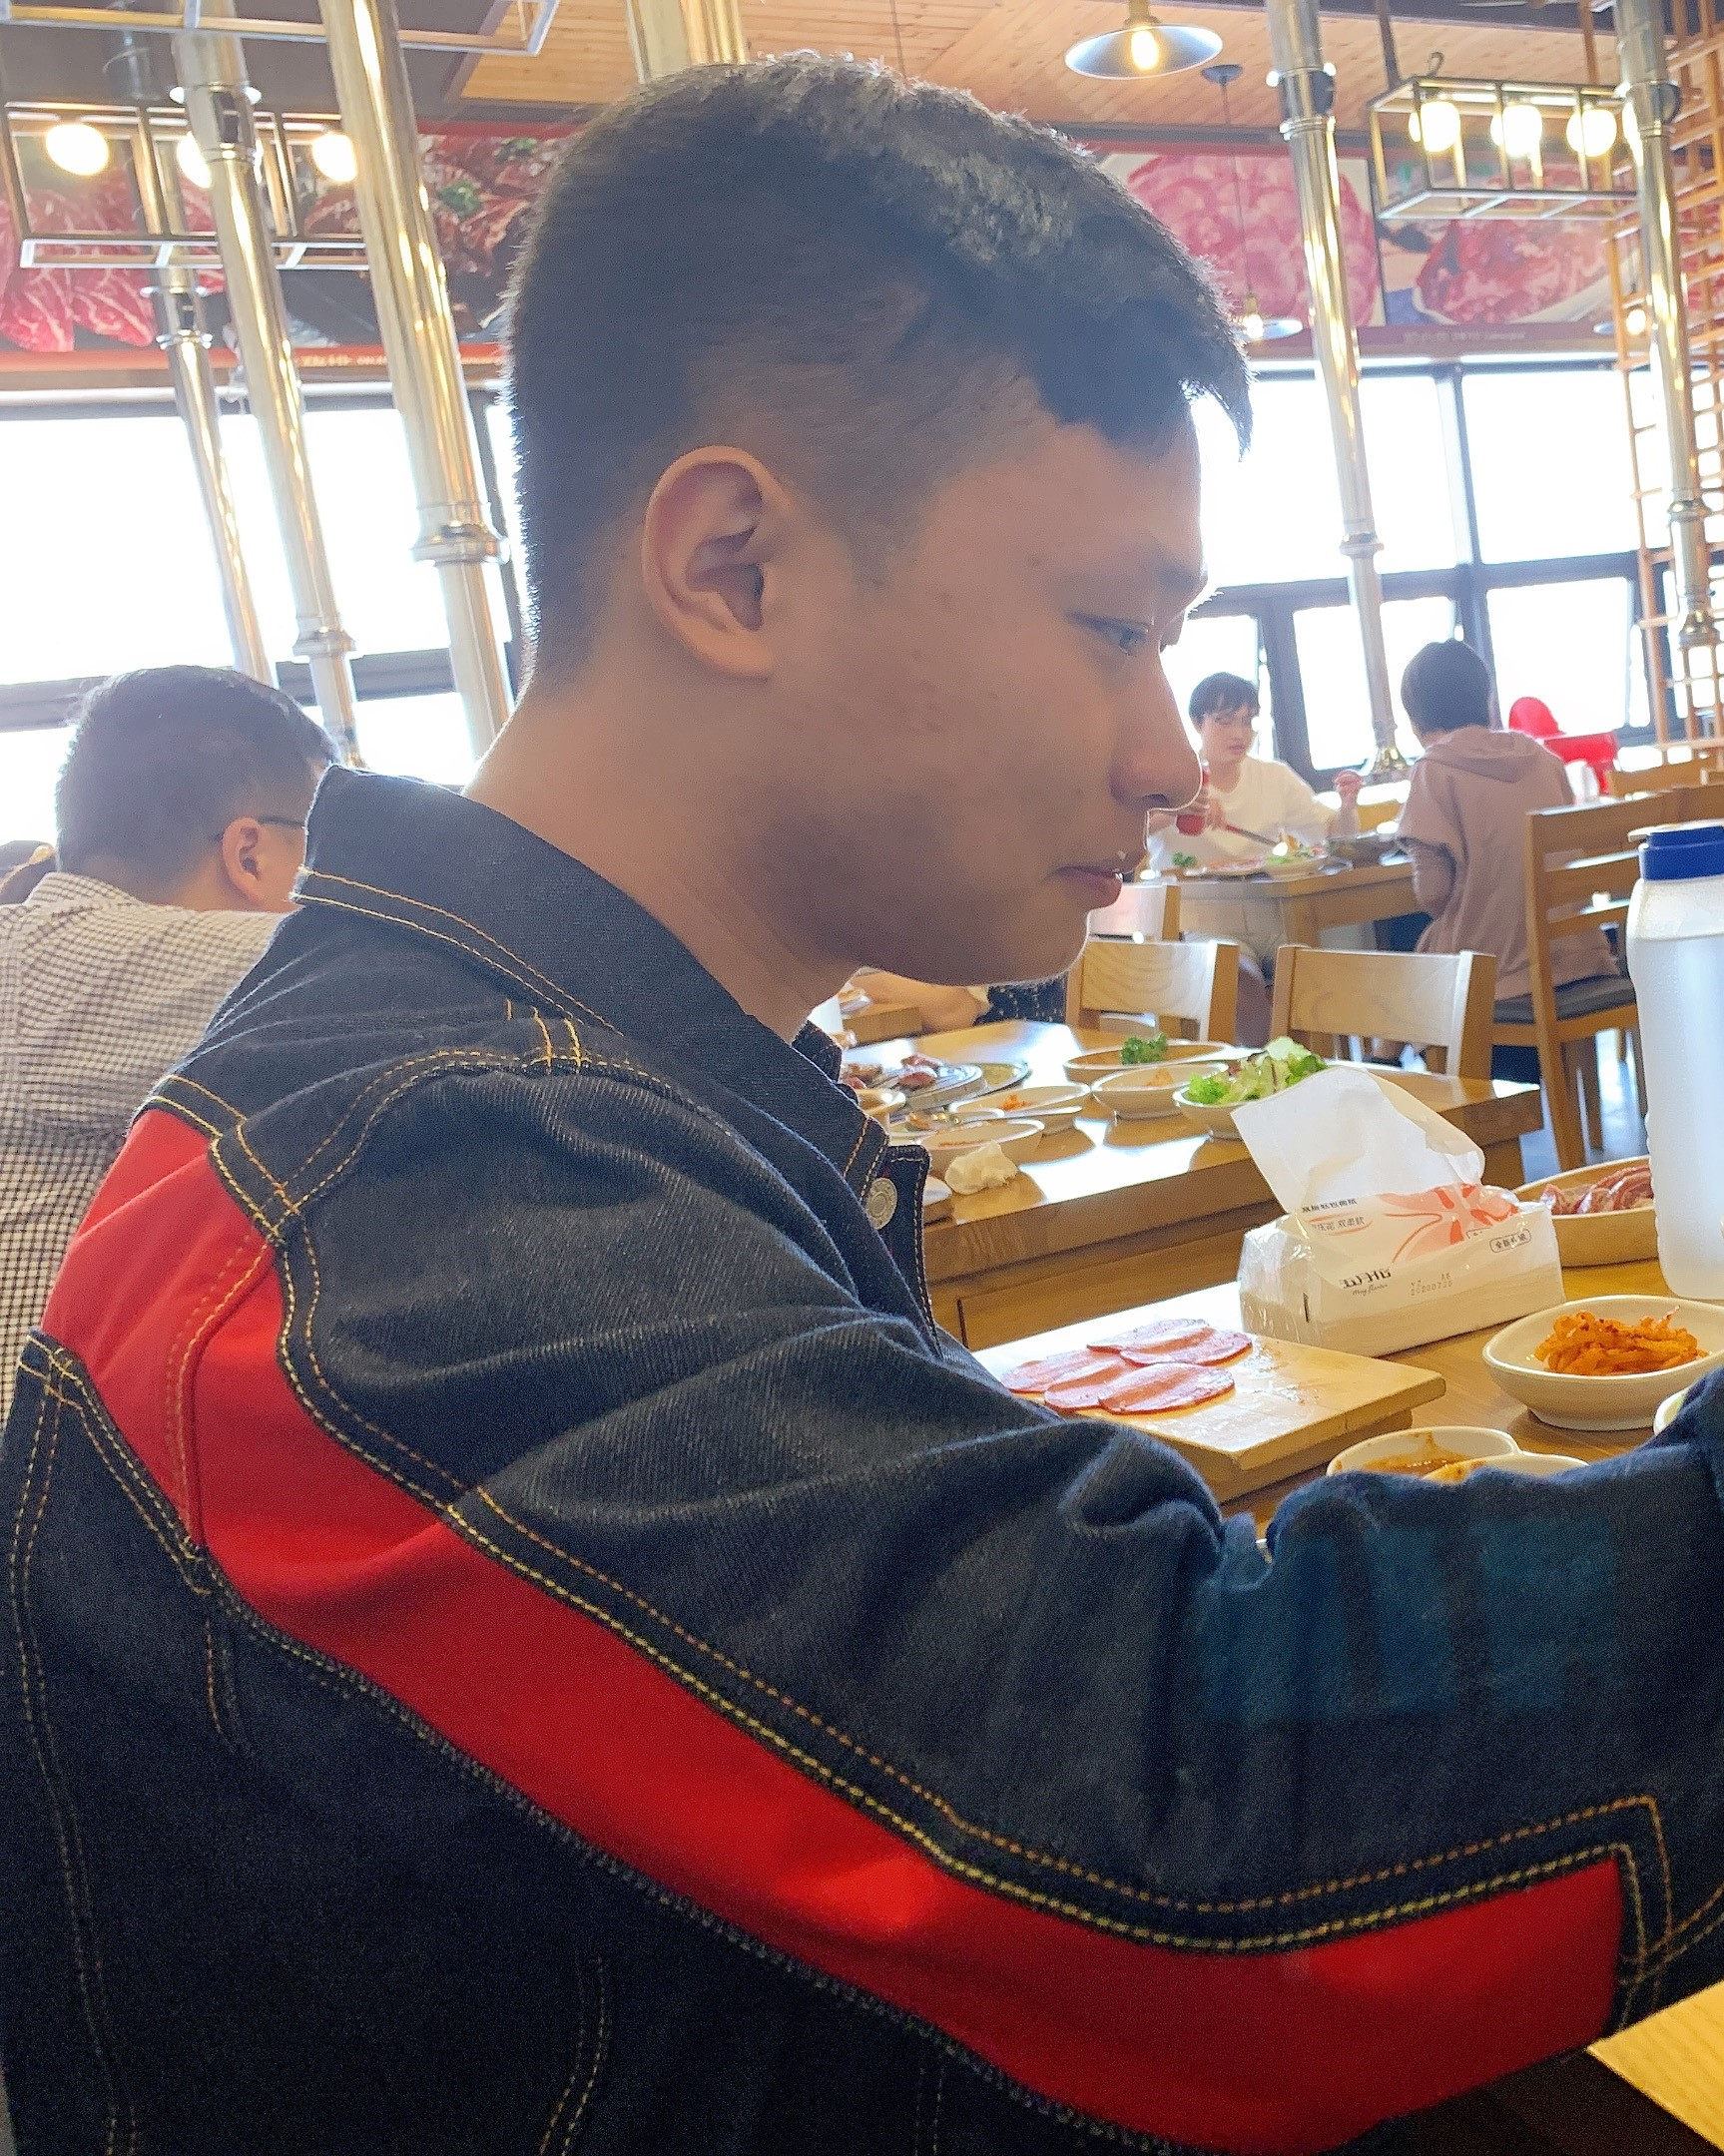
\includegraphics[width=70pt]{me.jpg}
\end{boxedminipage}
\end{wrapfigure}

\begin{tabular*}{0.5\textwidth}{l@{\extracolsep{\fill}}r}
  \textbf{{\huge 毕晓栋}} \\
    中国, 上海, 嘉定区, 曹安公路4800号, 201804 \\
    电话 :  +86\ 18616331732 \\
    邮箱: \href{mailto:bxddream@gmail.com}{bxddream@gmail.com} \\
\end{tabular*}

%-----------EDUCATION-----------------
\section{教育背景}
  \resumeSubHeadingListStart
    \resumeSubheading
      {同济大学电子信息与工程学院}{上海}
      {主修: 计算机科学与技术}{2017.09 至今}
      \resumeItemListStart
        \resumeItem{绩点:}{91.34/100.00,\ \ \textbf{GPA 排名:} 10.1\%\  (第16名/共159人),\ \ \textbf{综合排名:} 1.25\% (第2名/共159人)} 
        \resumeItem{相关课程:}{高级语言程序设计\ (优/优), 数据结构\ (优), 算法\ (优),  数据库原理\ (优), 操作系统\ (良), 计算机组成原理\ (优), 计算机体系结构\ (优), 计算机图形学\ (优),  人工智能\ (优), 模式识别\ (优), 数据挖掘\ (优), 机器学习\ (优), 多媒体技术\ (优)}
      \resumeItemListEnd
      \resumeSubheading
      {数学强化与计算机交叉培养实验区, 同济大学数学科学学院}{上海}
      {主修: 计算机科学与技术, 辅修: 数学}{2017.09-2019.01}
      \resumeItemListStart
      \resumeItem{绩点(大一上):}{4.37/5.00,\ \textbf{绩点(大一下):}4.81/5.00,\  \textbf{绩点(大二上):}4.78/5.00,\  \textbf{排名(计算机类):} 第1名/共15人} 
      \resumeItem{相关课程:}{数学分析\ (良/优), 高等代数\ (优/优), 数学实验\ (良/优), 概率论\ (优),
统计学\ (优), 数值分析\ (良), 数学建模\ (优), 常微分方程\ (优), 组合数学\ (优), 复变函数\ (优)}
      \resumeItemListEnd
  \resumeSubHeadingListEnd
  
\section{项目和经历}
  \resumeSubHeadingListStart
    \resumeSubheading
      {机器学习组, 微软亚洲研究院}{北京}
      {机器学习 研究实习生}{2020.06 至今}
      \resumeItemListStart
        \resumeItem{}{研究方向为机器学习在量化投资的应用,量化研究平台 \href{https://github.com/microsoft/qlib}{Qlib} 开源小组主要成员,获得超过4.9k Star。}
      \resumeItemListEnd
    \resumeSubheading
      {同济大学ACM程序设计竞赛暑期集训队}{上海}
      {队长, 组织者}{2019.06 - 2019.09}
      \resumeItemListStart
      \resumeItem{}
          {在叶晨教练的指导下, 举办网络算法讲堂, 为集训队进行算法的网络授课,并举办多次比赛训练集训队队员和选拔新队员。}
        \resumeItem{}
          {多次参加ACM-ICPC国际大学生程序大赛并获得优异成绩。}
      \resumeItemListEnd
    \resumeSubheading
      {\href{https://github.com/tiev-tongji/carla-ex}{同济途灵“TiEV”智能无人车研究团队}
      }{上海}
      {团队成员}{2020.01 至今}
      \resumeItemListStart
        \resumeItem{}
          {受副教授赵君峤和高级工程师叶晨指导。}
         \resumeItem{}
          {对无人车的训练环境进行模拟, 研究并开发了基于carla模拟器和GPU加速的激光雷达模拟器,并取得了很好的效果。}
         \resumeItem{}
          {极大优化了激光雷达的仿真性能, 大幅提高carla模拟器能支持的客户端的数目和激光雷达的仿真速度。}
      \resumeItemListEnd
    \resumeSubheading
      {\href{https://www.covestro.cn/zh-cn/media/news-releases/2019/covestro-holds-its-first-ever-international-data-science-hackathon-across-three-continents}{科思创国际数据分析马拉松应用设计大赛(Hackathon)}}{上海}
      {参赛者}{2019.11}
      \resumeItemListStart
        \resumeItem{}
          {使用基于长短时记忆网络(LSTM)的算法来预测莱茵河水位。}
          \resumeItem{}
          {基于历年降水监测站数据和历年水位来预测莱茵河的水位, 与卡内基梅隆大学和亚琛工业大学竞技, 成绩排名第一赛道第三。}
      \resumeItemListEnd
     \resumeSubheading
      {\href{https://github.com/ganler/bimulator}{Bimulator 开发团队}}{上海}
      {队长}{2019.10 - 2019.12}
      \resumeItemListStart
        \resumeItem{}
          {开发了基于物理引擎, 实时光线追踪和图形渲染管线的第一人称3D台球模拟器。
         }
         \resumeItem{}
         {使用box2D物理引擎来迷你台球碰撞的物理效果,实现了实时光线追踪, 使用光线追踪实现了反射和软阴影等视觉特效。
         }
      \resumeItemListEnd
  \resumeSubHeadingListEnd
  
 \section{获奖情况}
 \resumeSubHeadingListStart
     \resumeSubItem{银牌:}
     {ACM-ICPC国际大学生程序设计竞赛亚洲区决赛(The ACM-ICPC Asia-East Continent Final),}
    {2018.12}
    
    \resumeSubItem{金牌:}
    {ACM-ICPC中国大学生程序设计竞赛,\ 宁夏站(The ACM-ICPC Chinese Collegiate Programming Contest),}
    {2018.06}
    \resumeSubItem{金奖:}
    {CCF大学生计算机系统与程序设计竞赛\ 决赛 (2019 CCF CCSP),}
    {2019.10}
    \resumeSubItem{第一赛道第三:}
    {科思创国际数据分析马拉松应用设计大赛,}
    {2019.07}
    \resumeSubItem{荣誉:}
    {CCF 优秀大学生奖,}
    {2020.09}
    \resumeSubItem{荣誉:}
    {上海市优秀毕业生,}
    {2021.04}
    \resumeSubItem{省级三等奖:}
    {上海大学生数学建模竞赛,}
    {2018.09 \& 2019.09}
    \resumeSubItem{校级二等奖:}
    {同济大学数学建模竞赛,}
    {2018.05}
    \resumeSubItem{校级二等奖:}
    {同济大学程序设计竞赛暨上海大学生邀请锦标赛,}
    {2018.04}
    \resumeSubItem{校级二等奖学金:}
    {同济大学优秀学生奖学金,}
    {2018.12 \& 2019.12 \& 2020.12}
    \resumeSubItem{校级三等奖:}
    {同济大学非物理专业物理竞赛,}
    
 \resumeSubHeadingListEnd
%--------PROGRAMMING SKILLS------------
\section{语言和技能}
 \resumeSubHeadingListStart
 \resumeSubItem{语言能力:}{英语(大学英语六级)}
 \resumeSubItem{编程语言和框架:}{C/C++, Python, Matlab, Glsl, VerilogHDL, Pytorch, TensorFlow }
 \resumeSubItem{技能:}{
     熟悉机器学习和深度学习理论和编程实践, 模式识别和数据挖掘方法;
     熟练使用算法和数据结构优化程序的时间和空间复杂度;
     擅长数学; 熟悉计算机图形学, 并熟悉使用Mordern OpenGL编写程序;  熟练数据库查询操作; 熟悉多媒体技术。}
 \resumeSubHeadingListEnd
 
\end{spacing}
\begin{spacing}{1}
%----------HEADING-----------------
\begin{wrapfigure}[0]{r}{70pt}
\vspace{-35pt}
\begin{boxedminipage}{78pt}
\centering
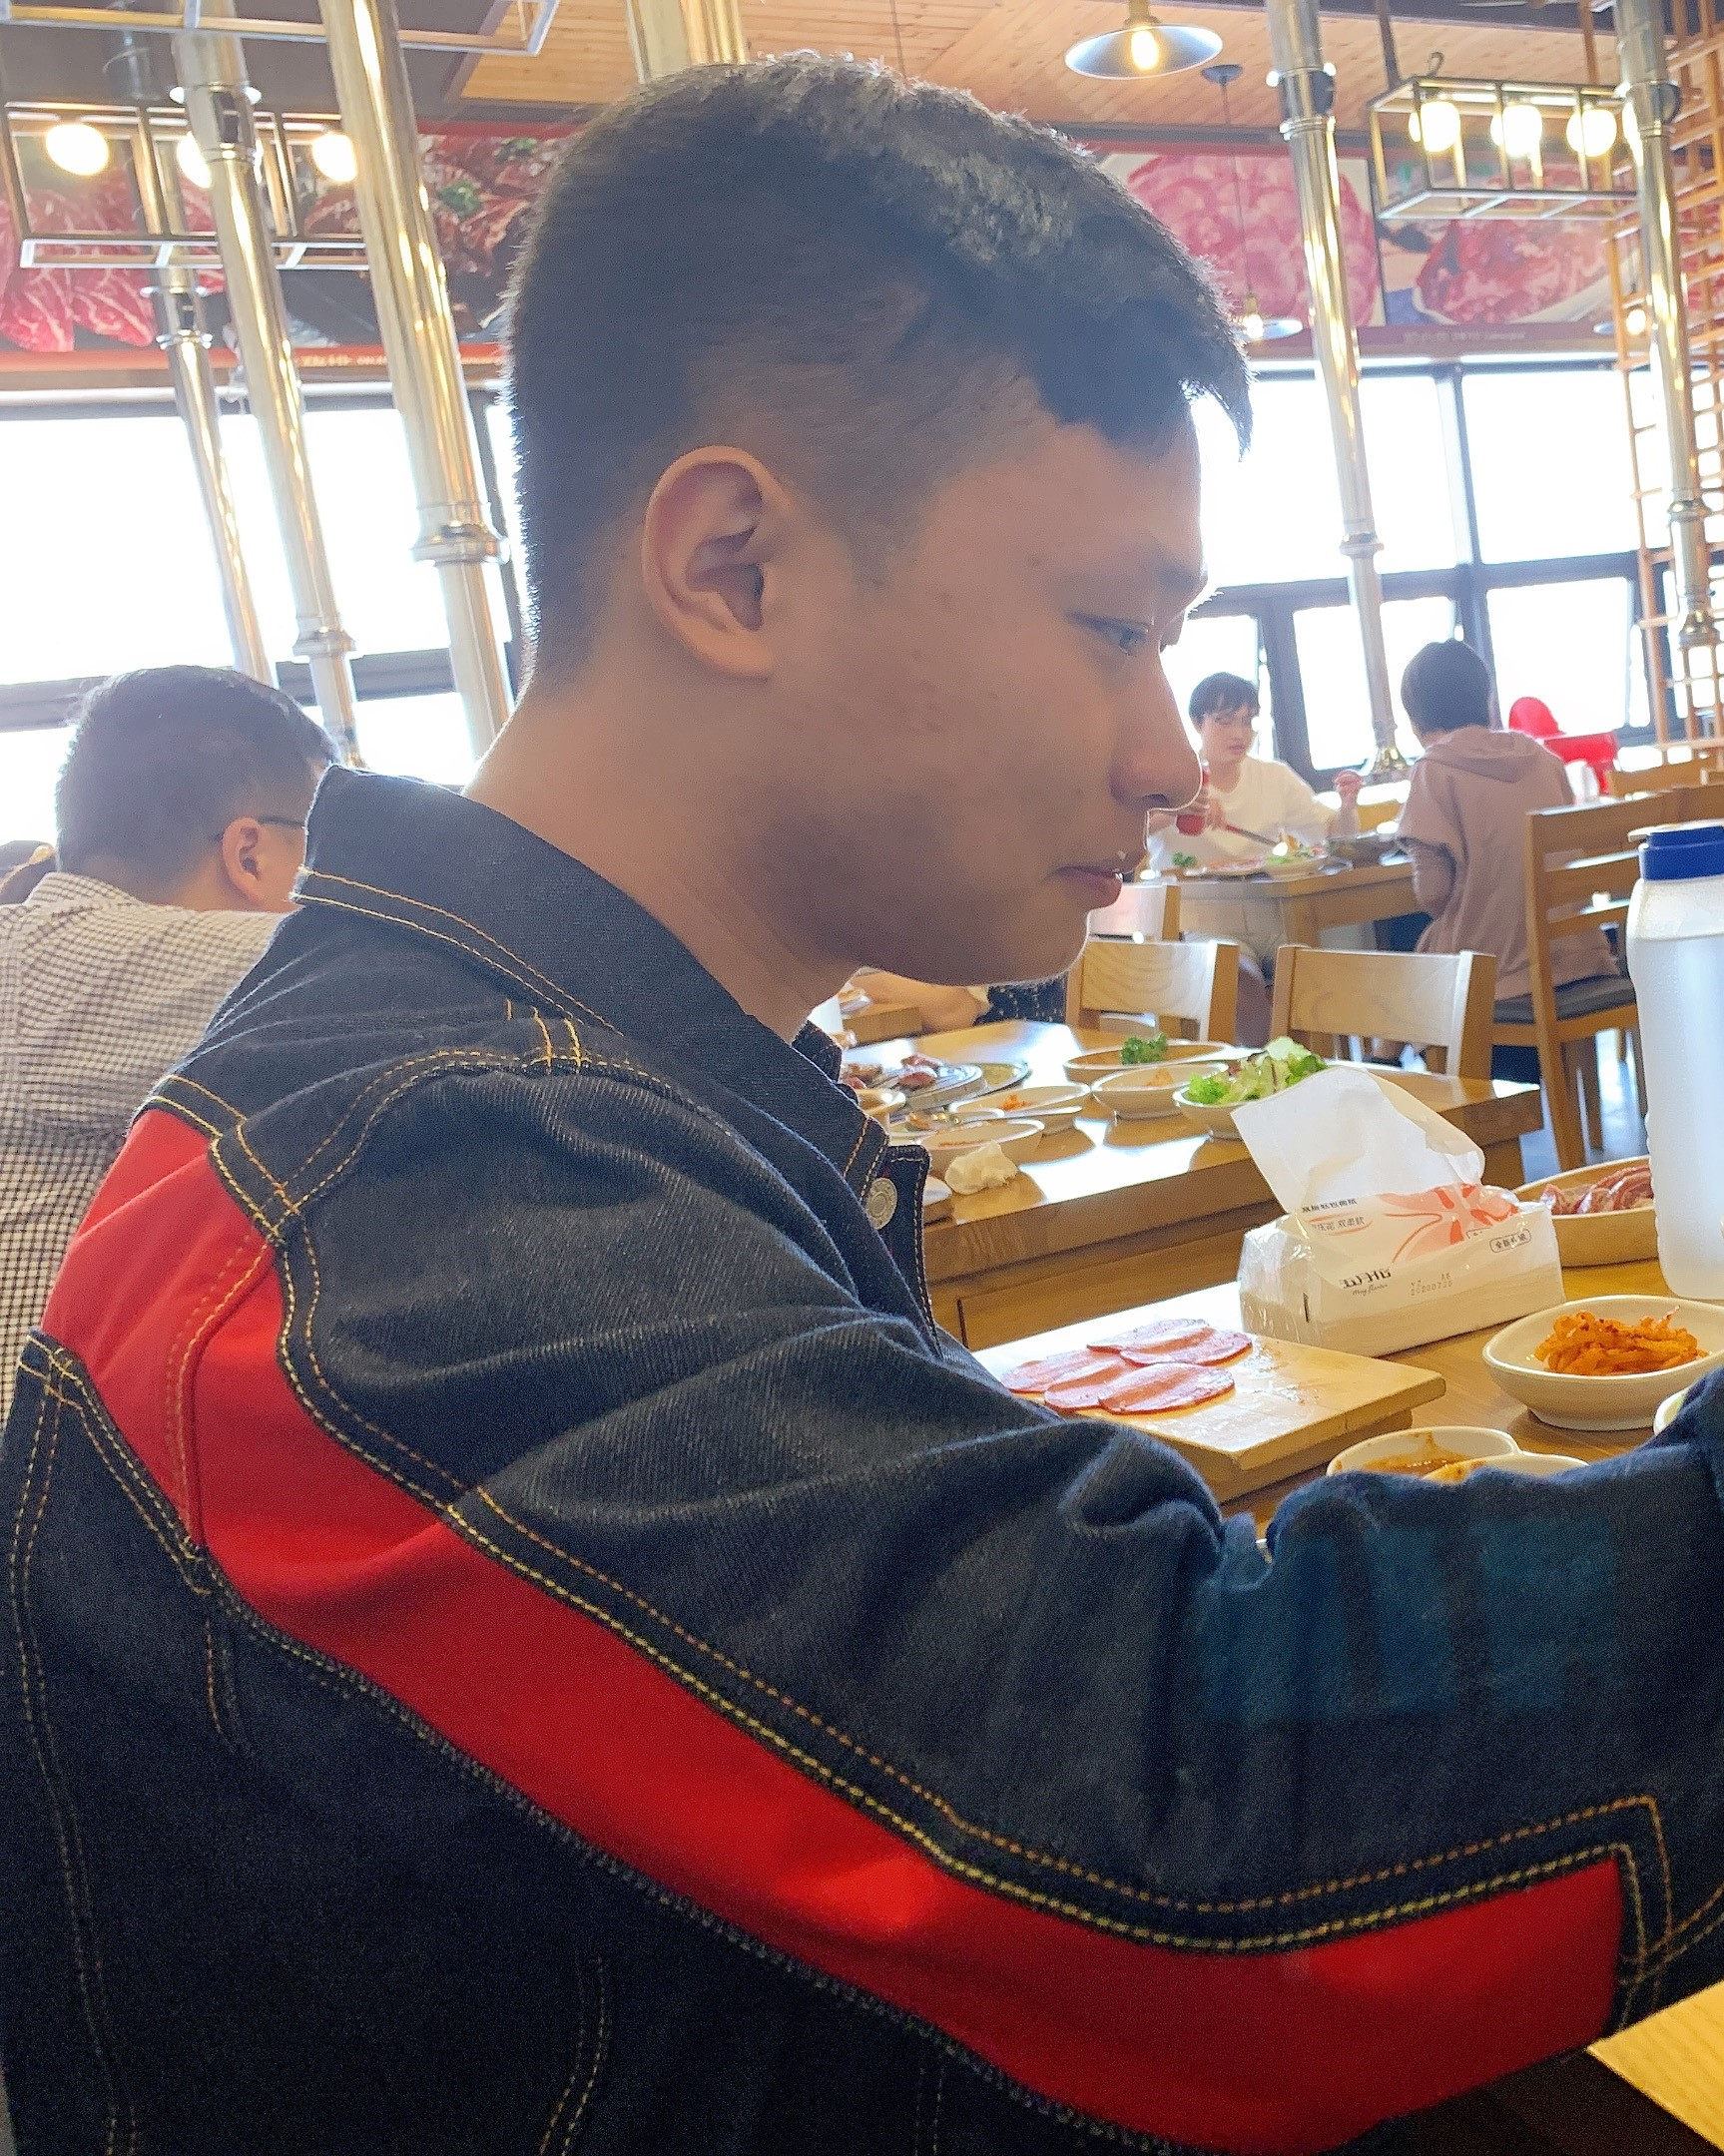
\includegraphics[width=70pt]{me.jpg}
\end{boxedminipage}
\end{wrapfigure}

\begin{tabular*}{0.5\textwidth}{l@{\extracolsep{\fill}}r}
  \textbf{{\huge Bi Xiaodong}} \\
    4800 Caoan Rd., Jiading Dist., Shanghai, China, 201804 \\
      Mobile :  +86\ 18616331732 \\
      Email : \href{mailto:bxddream@gmail.com}{bxddream@gmail.com} \\
\end{tabular*}



%-----------EDUCATION-----------------
\section{Education}
  \resumeSubHeadingListStart
    \resumeSubheading
      {College of Electronics and Information Engineering, Tongji University}{Shanghai}
      {Major: B.S. in Computer Science}{Sept. 2017 - Present}
      \resumeItemListStart
       \resumeItem{GPA:}{4.62/5.00,\ \ \textbf{GPA Ranking:} 10.1\%\  (16/159),\ \ \textbf{Comprehensive Ranking:} 1.25\%\  (2/159)} 
        \resumeItem{Course:}{Data Structures\ (A), Algorithm\ (A),  Principles of Database\ (A), Operating Systems\ (B), Computer Architecture\ (A), Computer Graphics\ (A),  Artificial Intelligence\ (A), Pattern Recognition\ (A), Data Mining\ (A), Machine Learning(A)}
      \resumeItemListEnd
      \resumeSubheading
      {Math Experimental Class, School of Mathematical Sciences, Tongji University}{Shanghai}
      {Major: B.S. in Computer Science Minor: B.S. in Mathematics}{Sept. 2017 - Jan. 2019}
      \resumeItemListStart
      \resumeItem{GPA($1^{st}$ term):}{4.37/5.00,\ \textbf{GPA($2^{nd}$ term):}4.81/5.00,\  \textbf{GPA($3^{rd}$ term):}4.78/5.00,\ \textbf{Rank:} 6.7\%\  (1/15)} 
      \resumeItem{Course:}{Mathematical Analysis\ (B/A), Advanced Algebra\ (A/A), Theory of Probability\ (A),
Statistics\ (A), Numerical Analysis\ (B), Mathematical Modeling\ (A), Ordinary Differential Equation\ (A), Combinatorics\ (A), Complex analysis\ (A)}
      \resumeItemListEnd
  \resumeSubHeadingListEnd
%-----------EXPERIENCE-----------------
\section{Project \& Experience}
  \resumeSubHeadingListStart
    \resumeSubheading
      {Machine Learning Group, Microsoft Research Asia}{Beijing}
      {Research Intern of Machine Learning}{Jun. 2020 - Present}
      \resumeItemListStart
        \resumeItem{}{Research the application of AI in quantitative investment, develop and maintain quant platform \href{https://github.com/microsoft/qlib}{Qlib} (4.9k Star).}
      \resumeItemListEnd


    \resumeSubheading
      {ACM Programming Summer Training Team of Tongji University}{Shanghai}
      {Captain and Organizer}{Jun. 2019 - Sept. 2019}
      \resumeItemListStart
      \resumeItem{}
          {Conducted online lectures and organized competitions to train and select members guided by A/Prof. Chen Ye.}
        \resumeItem{}
          {Participated in ICPC competitions many times and got good results.}
      \resumeItemListEnd
    \resumeSubheading
      {\href{https://github.com/tiev-tongji/carla-ex}{The 'TiEV' Research Group of Tongji Intelligent Electric Vehicle}
      }{Shanghai}
      {Developer and Researcher}{Jan. 2020 - Present}
      \resumeItemListStart
        \resumeItem{}
          {Guided by A/Prof. Junqiao Zhao. and A/Prof. Chen Ye.}
         \resumeItem{}
          {Research lidar simulator based on carla and GPU acceleration, and have achieved excellent results.}
         \resumeItem{}
         {Simulate the training environment of vehicles, optimize the lidar simulation frame rate by GPU acceleration.}
          
      \resumeItemListEnd
    \resumeSubheading
      {\href{https://www.covestro.cn/zh-cn/media/news-releases/2019/covestro-holds-its-first-ever-international-data-science-hackathon-across-three-continents}{Covestro International Data Science Hackathon}}{Shanghai}
      {Competitor}{Nov. 2019}
      \resumeItemListStart
        \resumeItem{}
          {Proposed an algorithm based on long short-term memory (LSTM) to predict the water level of the Rhine, achieved excellent results, and ranked $3^{rd}$ place in the first track.}
      \resumeItemListEnd
     \resumeSubheading
      {\href{https://github.com/ganler/bimulator}{Bimulator Development Team}}{Shanghai}
      {Team Leader}{Oct. 2019 - Dec. 2019}
      \resumeItemListStart
        \resumeItem{}
          {Developed a 3D billiard simulator using physics engine, ray tracing and graphics pipeline.
         }
         \resumeItem{}
         {Implemented real-time ray tracing, and use ray tracing to achieve reflection and soft shadow effects}
      \resumeItemListEnd
  \resumeSubHeadingListEnd
  
 \section{Awards}
 \resumeSubHeadingListStart
    \resumeSubItem{Silver Medal:}
    {The ACM-ICPC Asia-East Continent Final,}
    {Dec. 2018}
    \resumeSubItem{Gold Medal:}
    {The ACM-ICPC Chinese Collegiate Programming Contest, NingXia Site,}
    {Jun. 2018}
    \resumeSubItem{Gold Medal:}
    {The CCF College Computer Systems \& Programming Contest (2019 CCF CCSP),}
    {Oct. 2019}
    \resumeSubItem{$3^{rd}$ Place in the First Track:}
    {Covestro International Data Science Hackathon,}
    {July 2019}
    \resumeSubItem{Honour:}
    {CCF Elite Collegiate Student Award,}
    {Sept. 2020}
    \resumeSubItem{Honour:}
    {Outstanding Graduate in Shanghai,}
    {Apr. 2021}
    \resumeSubItem{$3^{rd}$ Province-Level Prize:}
    {Contemporary Undergraduate Mathematical Contest in Modeling,}
    {Sept. 2018/2019}
    \resumeSubItem{$2^{nd}$ Prize:}
    {Mathematical Modeling Contest of Tongji University,}
    {May. 2018}
    \resumeSubItem{$2^{nd}$ Prize:}
    {Tongji University Programming Competition,Shanghai University Invitational Tournament,}
    {Apr. 2018}
    \resumeSubItem{Second-Class Scholarship:}
    {Tongji University Outstanding Student Scholarship,}
    {Dec. 2018/2019/2020}
    
    \resumeSubItem{$3^{nd}$ Prize}
    {Physics Competition for non-Physics Major Students of Tongji University,}
    {June. 2018}
 \resumeSubHeadingListEnd
%--------PROGRAMMING SKILLS------------
\section{Languages \& Skills}
 \resumeSubHeadingListStart
 \resumeSubItem{Languages:}{Mandarin(Native), English(CET6)}
 \resumeSubItem{Programming Languages and Frameworks:}{:C/C++, Python, Matlab, Glsl, VerilogHDL, Pytorch, TensorFlow}
 \resumeSubItem{Skills:}
 {Familiar with machine learning, deep learning, pattern recognition and data mining; Familiar with data structures and algorithms; Good at maths; Familiar with computer graphics and Modern OpenGL; Familiar with multimedia technology.}
\clearpage
 \resumeSubHeadingListEnd
\end{spacing}

\end{document}
